\section{Experiments}
\label{sec:experiments}

\subsection{Setup and Comparison Protocol}
\label{sec:setup}

Unless otherwise specified, all main LSD experiments use the training-time routing threshold $\tau=1$. Full configurations are in Appendix~\ref{app:experimental-configurations}.

\paragraph{Single-Turn Reasoning Task.}
We post-train Qwen3-4B-Base on deduplicated DAPO-Math-17K and evaluate AMC 2023 and AIME 2025--2026 with 32 responses per query and a 4k response budget. We compare RL, the three LSD variants, CRISP~\citep{sang2026opsdc}, and Fixed SG-FKL. CRISP distills a periodically refreshed, concise-prompted teacher using reverse KL on all rollouts. Fixed uses a frozen $\pi_0$ teacher, a fixed routing map with threshold 1, and an LSD coefficient of 1. SG-FKL and SG-RKL use $K=32$; EMA updates start after four actor updates. Fixed-easy-set evaluation thresholds are separate from the training routing threshold.

\paragraph{Multi-Turn Agentic Task.}
We follow~\citet{wu2025cutbill} and post-train Qwen3-8B-Base on the CutTheBill training split, evaluating it on BrowseComp-Plus~\citep{chen2025browsecomp}. We use a 20,000-token response budget, at most 48 turns, and a separate Qwen3-8B refinement agent. We compare RL, the three LSD variants, and RL + Length Penalty under the same environment and evaluation configuration. Following AdapThink~\citep{xu2026adapthink}, RL + Length Penalty applies stronger length penalties to easier queries. We report Pass@1, average turns, and $\mathrm{LST}_{50}$. For the agent setting, response length in Eq.~\ref{eq:lst} is the sum of policy-generated tokens across turns; tool observations and refinement-model generation are separate cost components.

\subsection{Main Results}
\label{sec:main-results}
\label{sec:single-turn}

\begin{figure}[ht]
  \centering
  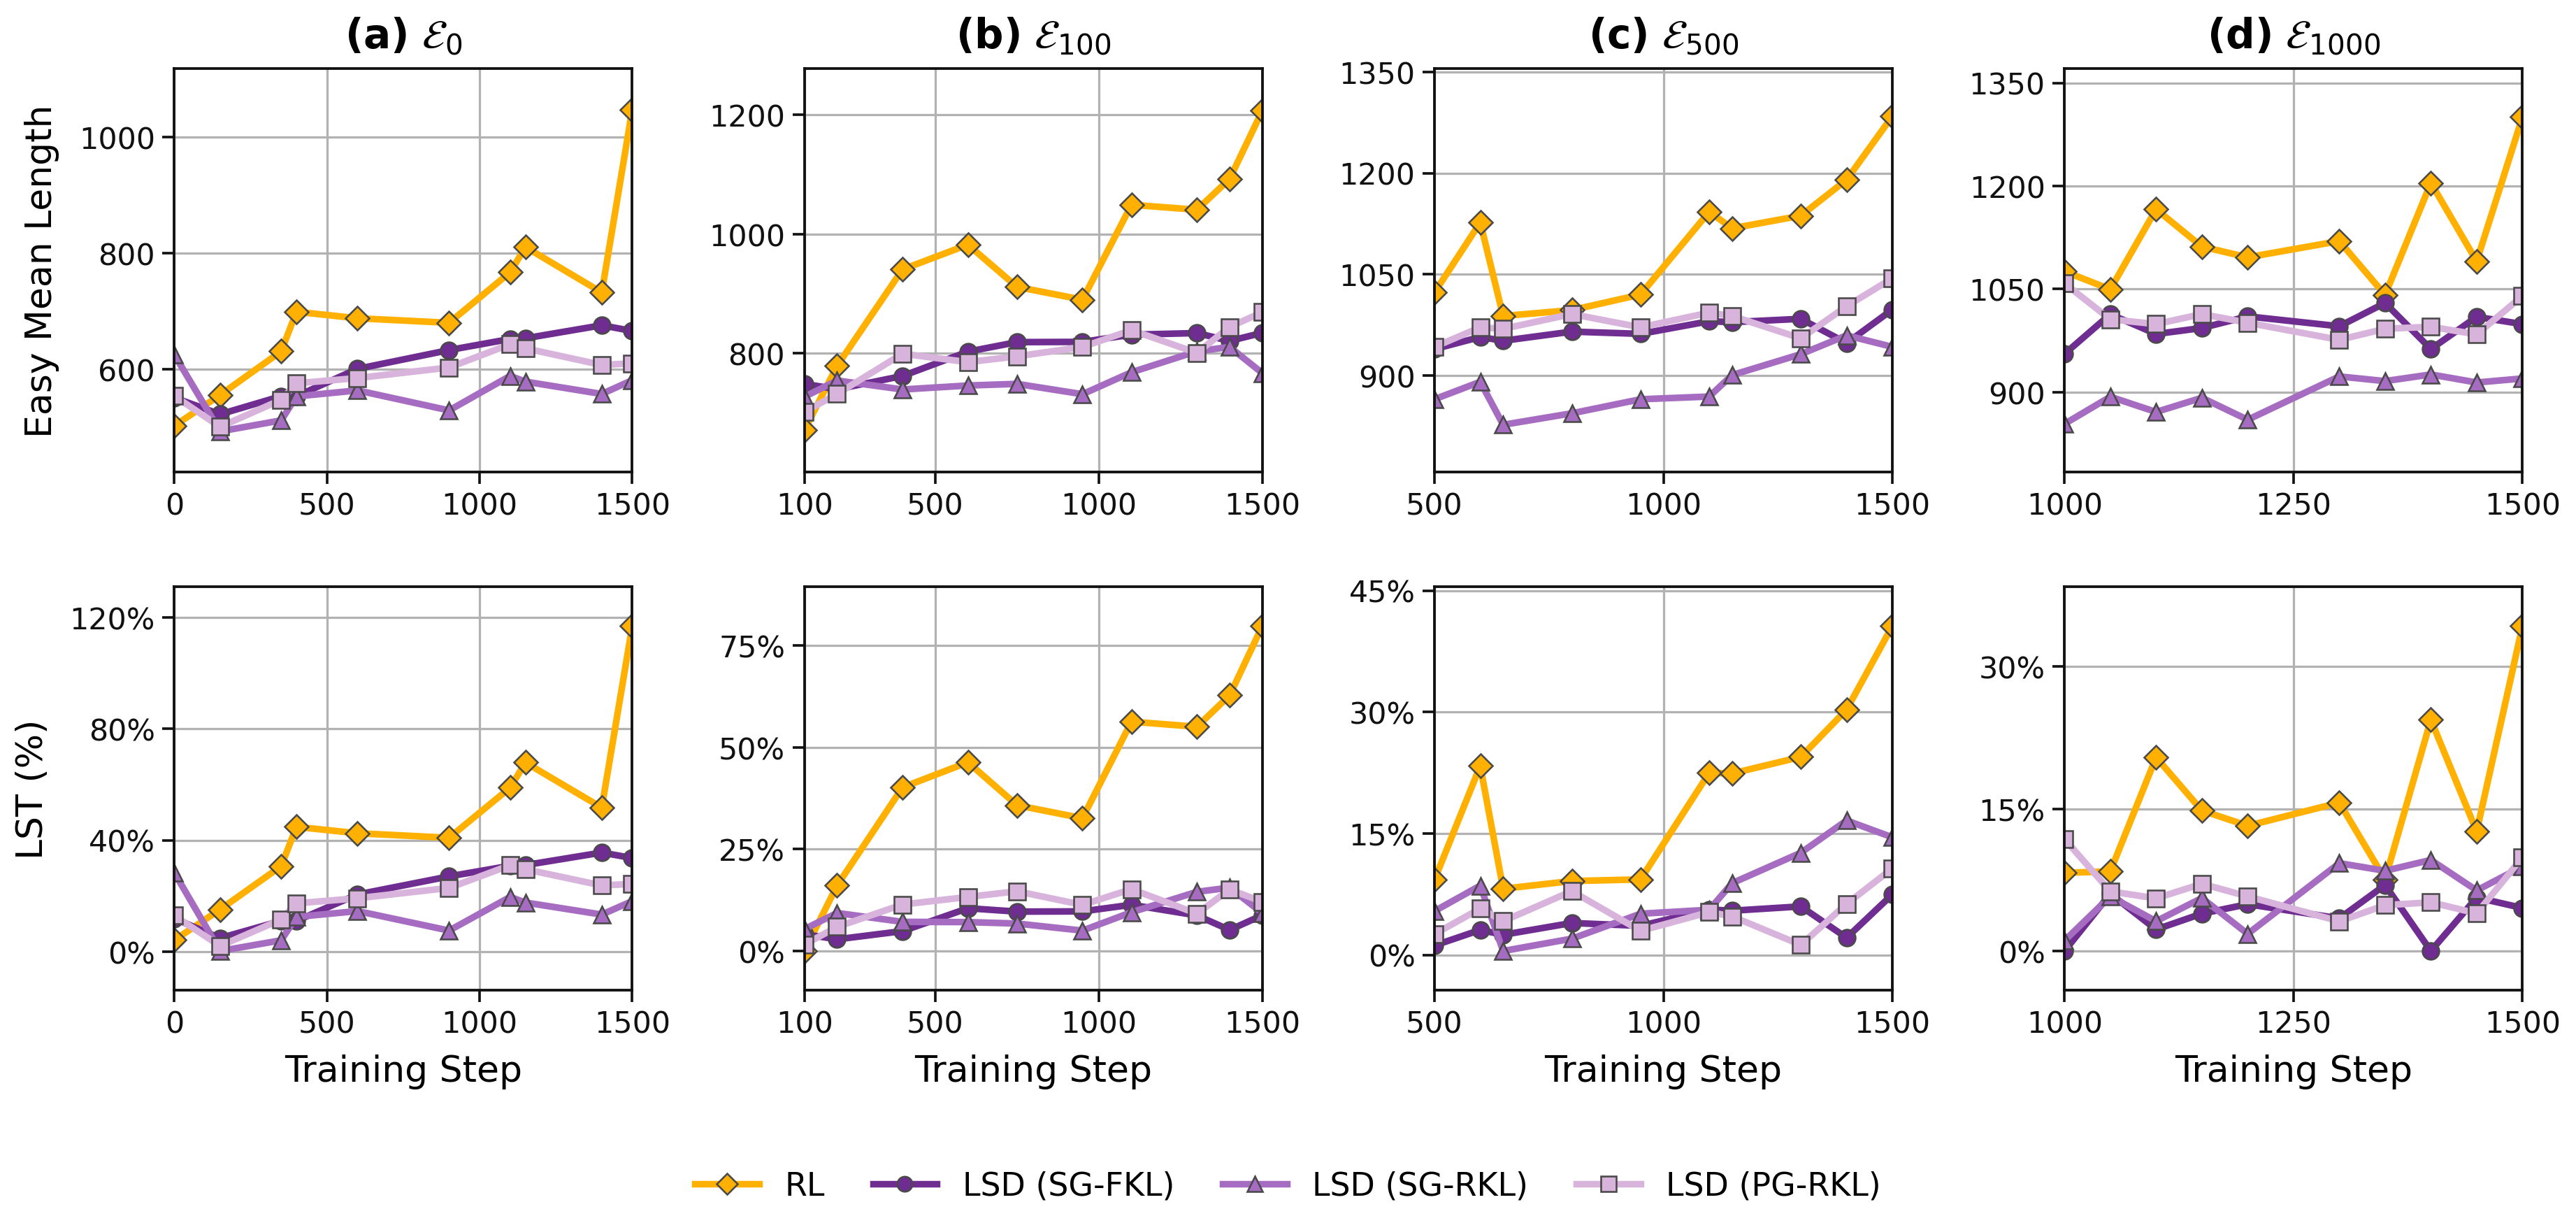
\includegraphics[width=0.90\linewidth]{figures/easy_tracking_v1.png}
  \caption{\textbf{Length growth on fixed easy queries.} Across four anchor-defined sets, all three LSD variants have lower easy-query length and LST than RL through most of training. The upper panels report mean length and the lower panels report LST. Different anchors select different cohorts.}
  \label{fig:lsd-easy-tracking}
\end{figure}

\paragraph{Maintaining concise reasoning on easy queries.}
Figure~\ref{fig:lsd-easy-tracking} shows that LSD curbs easy-query length growth across anchors. Appendix~\ref{app:paired-preservation} jointly reports accuracy and length on identical frozen query sets. Quantitatively, Figure~\ref{fig:lsd-selected-summary} and Table~\ref{tab:lsd-best-each-max} show that, on single-turn reasoning, $\mathrm{LST}_{1000}$ decreases from \mainLSTRLShort\% under RL to \mainLSTFKLShort\%, \mainLSTRKLShort\%, and \mainLSTPGShort\% under SG-FKL, SG-RKL, and PG-RKL, respectively. \label{sec:agent}The same pattern extends to multi-turn agentic tasks. As reported in Figure~\ref{fig:agent-main} and Table~\ref{tab:agent-main-results} in Appendix~\ref{app:benchmark}, $\mathrm{LST}_{50}$ decreases from 31.4\% under RL to 13.7\%, 9.2\%, and 16.1\% under SG-FKL, SG-RKL, and PG-RKL, respectively.

\begin{figure}[ht]
  \centering
  \begin{subfigure}[t]{0.49\linewidth}
    \centering
    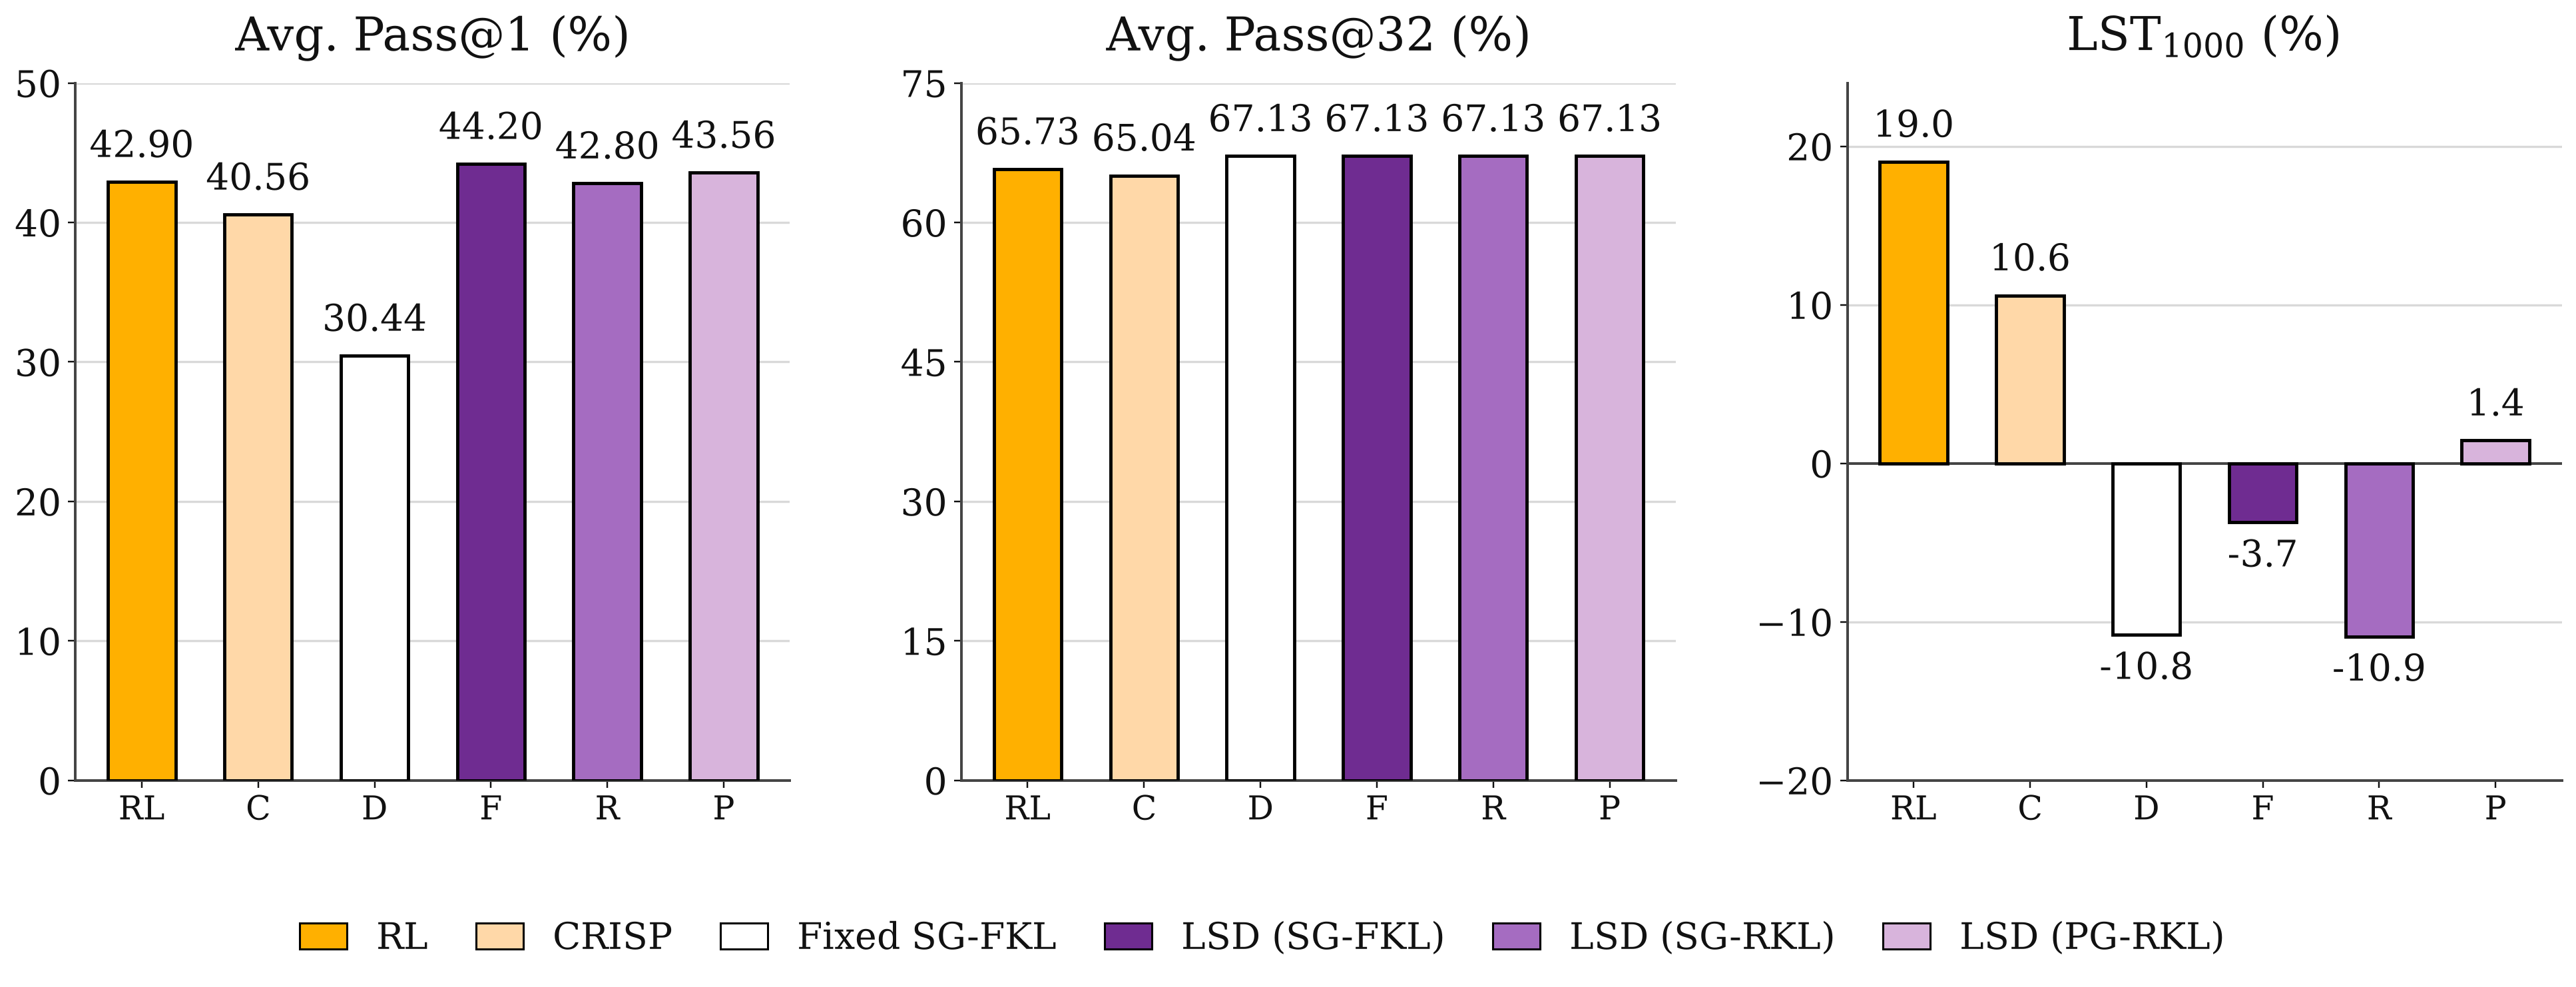
\includegraphics[width=\linewidth]{figures/lsd_single_all.png}
    \caption{Single-turn reasoning tasks.}
    \label{fig:lsd-selected-summary}
  \end{subfigure}\hfill
  \begin{subfigure}[t]{0.49\linewidth}
    \centering
    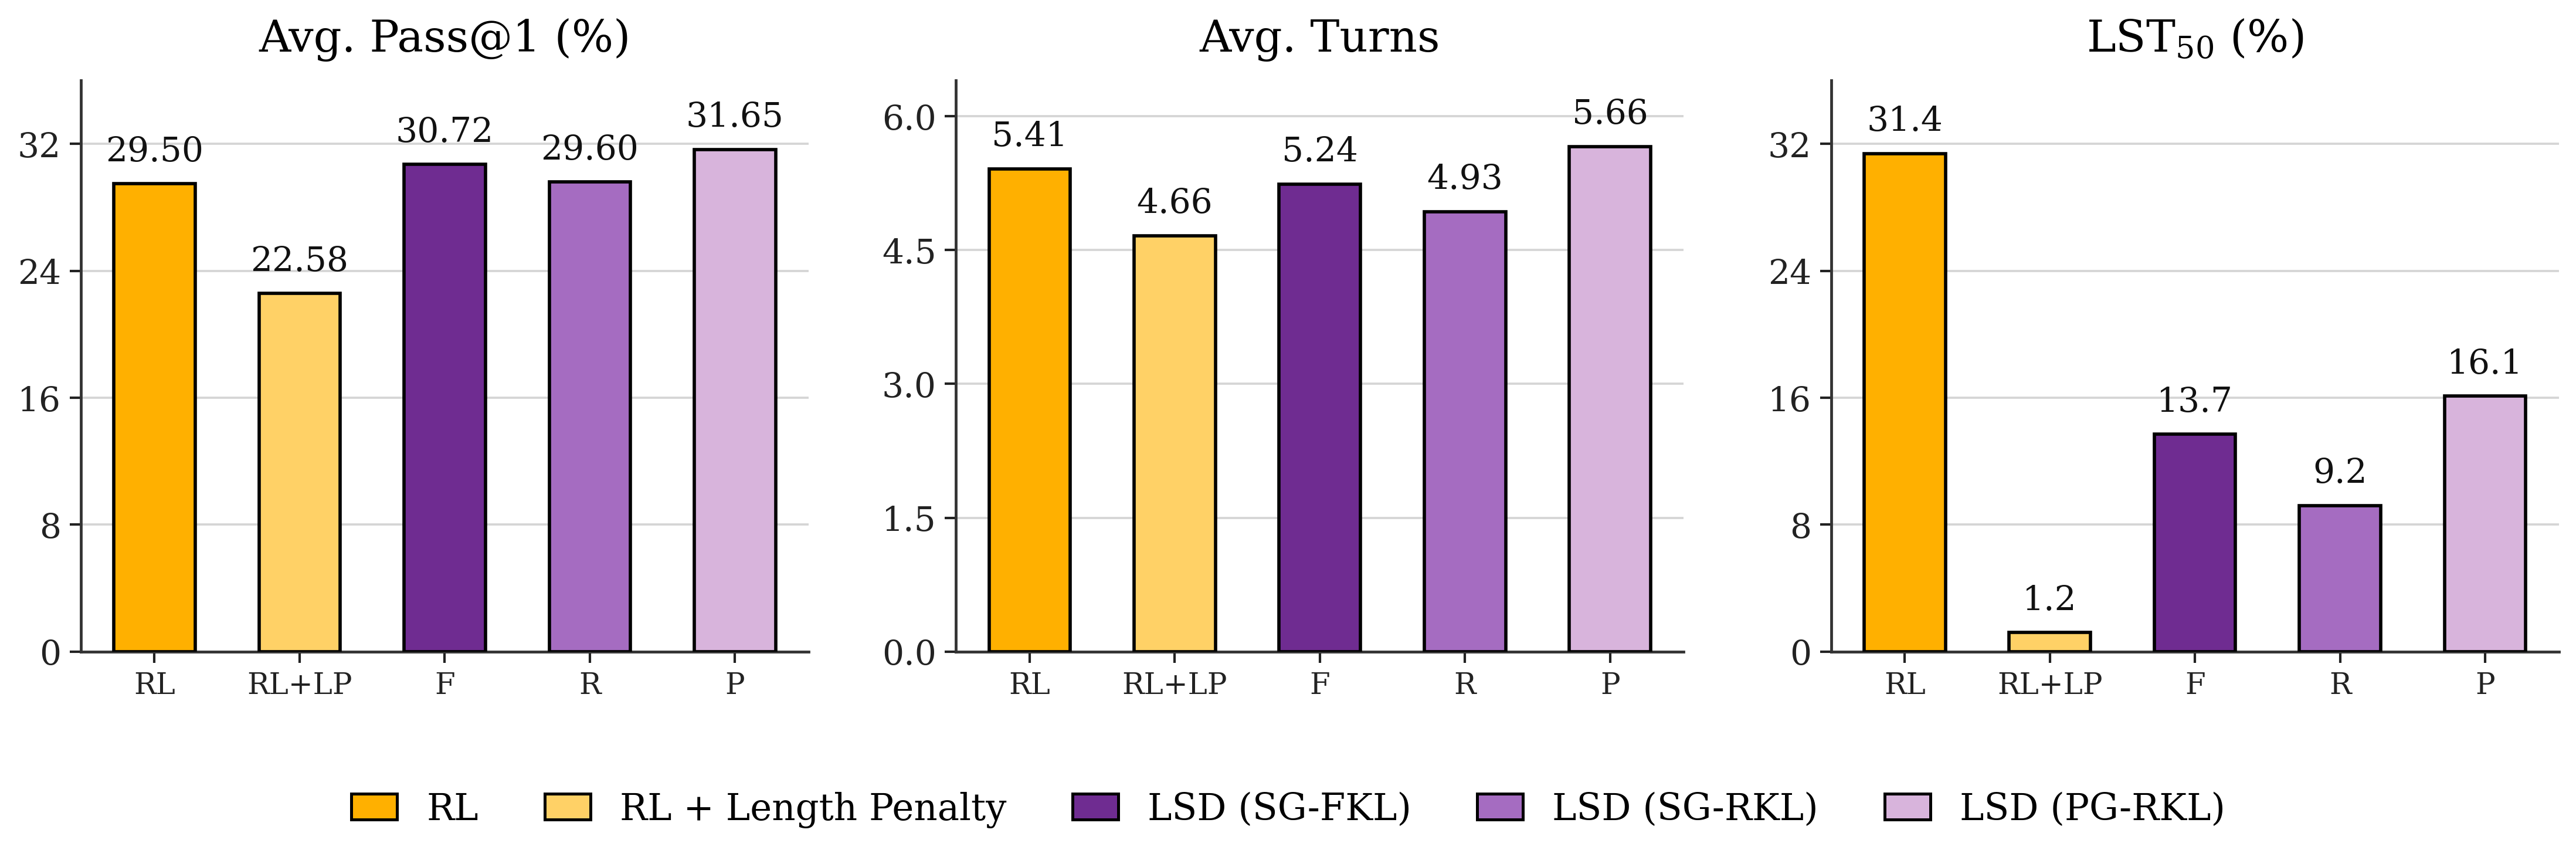
\includegraphics[width=\linewidth]{figures/avg_pass1_avg_turns_lst50.png}
    \caption{Multi-turn agentic tasks.}
    \label{fig:agent-main}
  \end{subfigure}
  \caption{\textbf{Capability and length-scaling tax across tasks.} (a) Single-turn average Pass@1, Pass@32, and $\mathrm{LST}_{1000}$. (b) BrowseComp-Plus average Pass@1, turns, and $\mathrm{LST}_{50}$. C and D denote CRISP and Fixed SG-FKL; F, R, and P denote LSD with SG-FKL, SG-RKL, and PG-RKL. RL+LP denotes RL + Length Penalty.}
  \label{fig:main-comparison}
\end{figure}

\paragraph{Encouraging more reasoning on hard queries.}
The reduction in easy-query length does not extend to the hard-query cohort. Table~\ref{tab:lsd-best-each-max} reports results on a fixed easy-query set and its hard-query complement. Average hard-query length increases from 2329 tokens under RL to 2511, 2395, and 2393 tokens under SG-FKL, SG-RKL, and PG-RKL, respectively. All three variants therefore produce shorter responses on easy queries while allowing longer responses on hard queries.

The training allocation shows a complementary pattern. As shown in Figure~\ref{fig:training-token-routes}, during training after step 500, the easy route accounts for only 12.17\%, 10.58\%, and 10.94\% of tokens under SG-FKL, SG-RKL, and PG-RKL, respectively. The hard route therefore retains 87.83--89.42\% of the logged token share on average. This allocation keeps training primarily focused on hard queries while preserving concise response patterns on easy queries.

\paragraph{Comparing efficiency baselines.}
CRISP yields 40.56\% Pass@1; Fixed SG-FKL yields 30.44\% Pass@1 and \mainLSTFixedShort\% $\mathrm{LST}_{1000}$ (Figure~\ref{fig:lsd-selected-summary}; Table~\ref{tab:lsd-best-each-max}). On multi-turn tasks, RL + Length Penalty reduces $\mathrm{LST}_{50}$ to 1.2\% and average turns to 4.66, but lowers Pass@1 to 22.58\% (Table~\ref{tab:agent-main-results}).

\paragraph{Comparing the three KL objectives.}
Overall, the three KL objectives differ in how strongly they preserve existing behavior and how they distribute probability across candidate responses. Their Pass@1 scores vary slightly, while their Pass@32 scores are nearly identical. Among the three EMA variants, SG-RKL achieves the lowest LST, but its stronger easy-query compression accompanies lower Pass@1.

The loss definitions offer a possible explanation. SG-FKL weights discrepancies by teacher probabilities, whereas SG-RKL penalizes student mass on tokens assigned low teacher probability. With a lagged teacher, the latter may more strongly preserve established behavior. As shown in Figure~\ref{fig:objective-training-dynamics} and Table~\ref{tab:objective-training-diagnostics}, SG-RKL has lower mean actor entropy (0.0367) than SG-FKL (0.0743) and PG-RKL (0.0542), together with the smallest mean absolute teacher--rollout log-probability difference before updates. Meanwhile, PG-RKL updates sampled actions using the original token probabilities, whereas SG-RKL directly optimizes distributions renormalized on the retained support. This distinction may also contribute to their different outcomes.

\subsection{Ablations}
\label{sec:ablations}

In this section, we ablate two additional hyperparameters introduced by LSD: the EMA half-life $H$ and the routing threshold $\tau$. All ablations use the SG-FKL variant, which achieves the highest average Pass@1 on single-turn reasoning among the three LSD variants.

\paragraph{EMA half-life.}
Figure~\ref{fig:ablation-half-life} compares $H\in\{2,4,8\}$ with $\tau=1$. A longer half-life generally suppresses LST but slows capability acquisition. Among the tested settings, $H=4$ achieves the highest average Pass@1 (41.85\%) at step 1750 (Table~\ref{tab:ablation-endpoints}), indicating that keeping the teacher closer to the online policy is not always beneficial. As shown in Figure~\ref{fig:half-life-training-diagnostics} and Table~\ref{tab:ablation-training-diagnostics}, we compare teacher--student parameter lag, distillation loss, and token routing across half-lives. Larger $H$ produces a greater parameter lag and higher distillation loss, while a smaller share of tokens is routed to OPD. The intermediate lag at $H=4$ may provide a stable behavioral reference while allowing the teacher to track improvements in the online policy.

\begin{figure}[!ht]
  \centering
  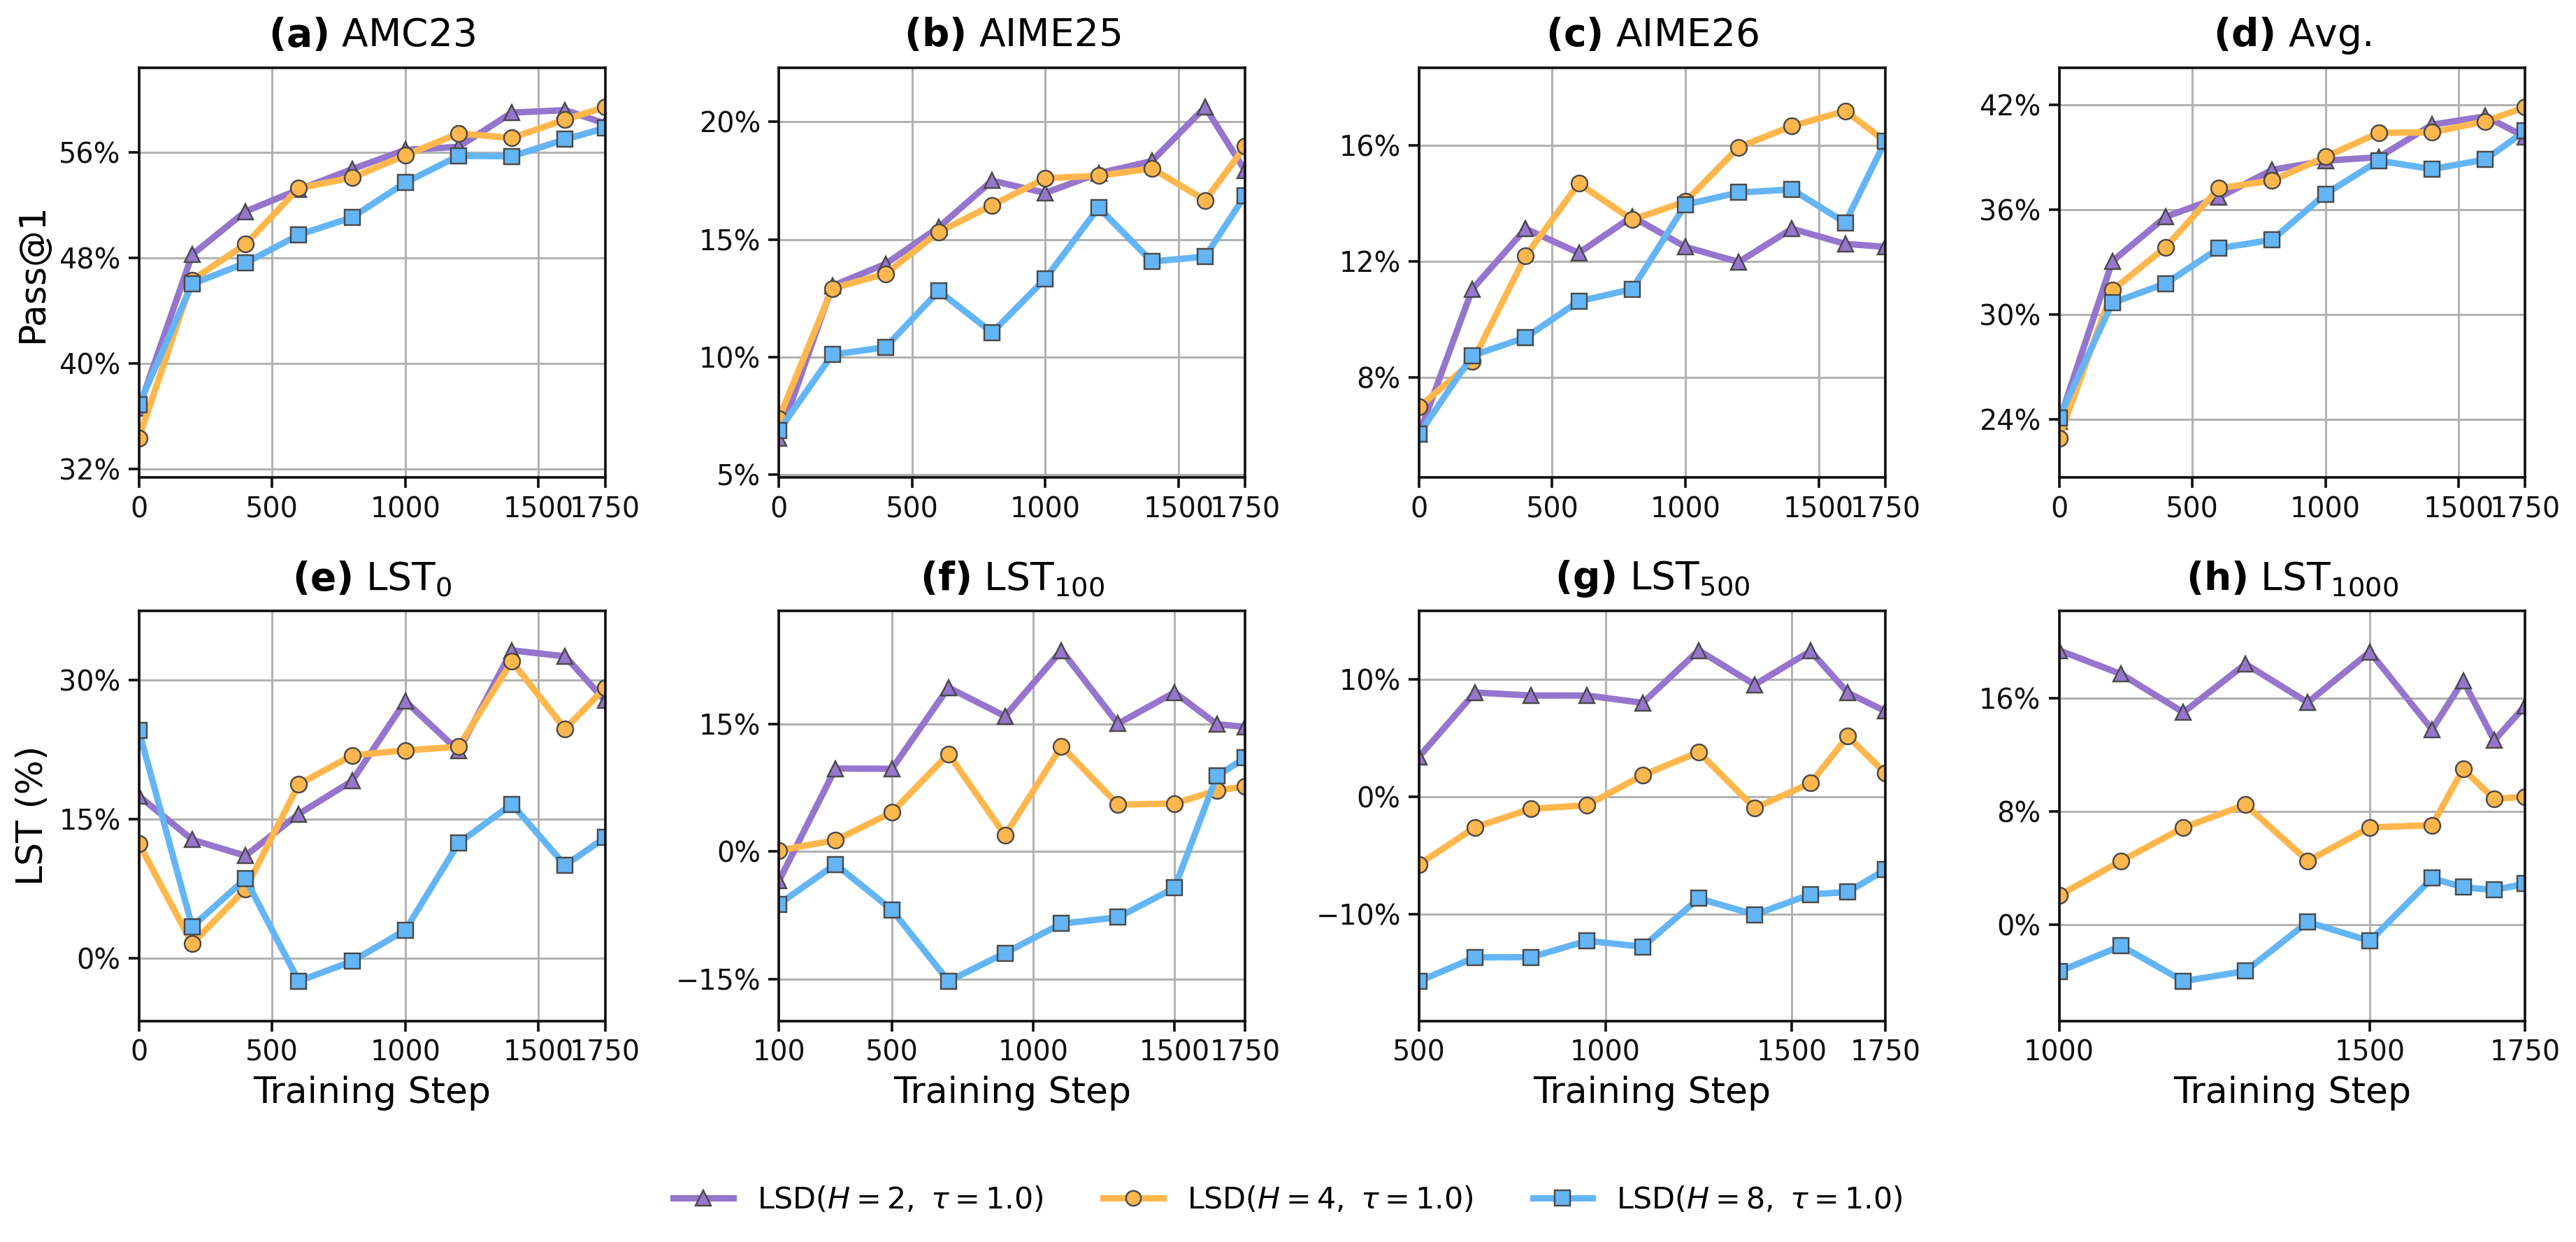
\includegraphics[width=0.78\linewidth]{figures/ablation_hl.png}
  \caption{\textbf{EMA half-life ablation.} We compare $H=2,4,8$ at $\tau=1.0$ through step 1750. The upper row shows benchmark and aggregate Pass@1; the lower row shows LST for anchors $b=0,100,500,1000$. }
  \label{fig:ablation-half-life}
\end{figure}

\paragraph{Scope of difficulty routing.}
We examine whether preservation should extend to partially solved queries by varying $\tau\in\{1.0,0.85,0.75\}$ with SG-FKL and $H=4$. Lowering $\tau$ routes more partially solved groups to distillation. At step 1750, average Pass@1 decreases from 41.85\% to 40.91\% and 39.31\%, respectively (Figure~\ref{fig:ablation-threshold}; Table~\ref{tab:ablation-endpoints}). Meanwhile, the mean distillation token share increases from 10.31\% to 19.00\% (Figure~\ref{fig:threshold-training-diagnostics}; Table~\ref{tab:ablation-training-diagnostics}). These results support restricting preservation to fully solved rollout groups: such groups lack a group-relative reward signal, whereas partially solved groups still provide reward variation for continued RL learning. Extending preservation before rollout accuracy saturates can therefore compromise capability acquisition. Moreover, to assess the role of query selection, we compare LSD with count-matched random routing under the same EMA and distillation settings (Appendix~\ref{app:paired-preservation}, Table~\ref{tab:paired-main-easy-set}). See Appendix~\ref{app:ablations} for the interpretation of negative LST values.

\begin{figure}[!ht]
  \centering
  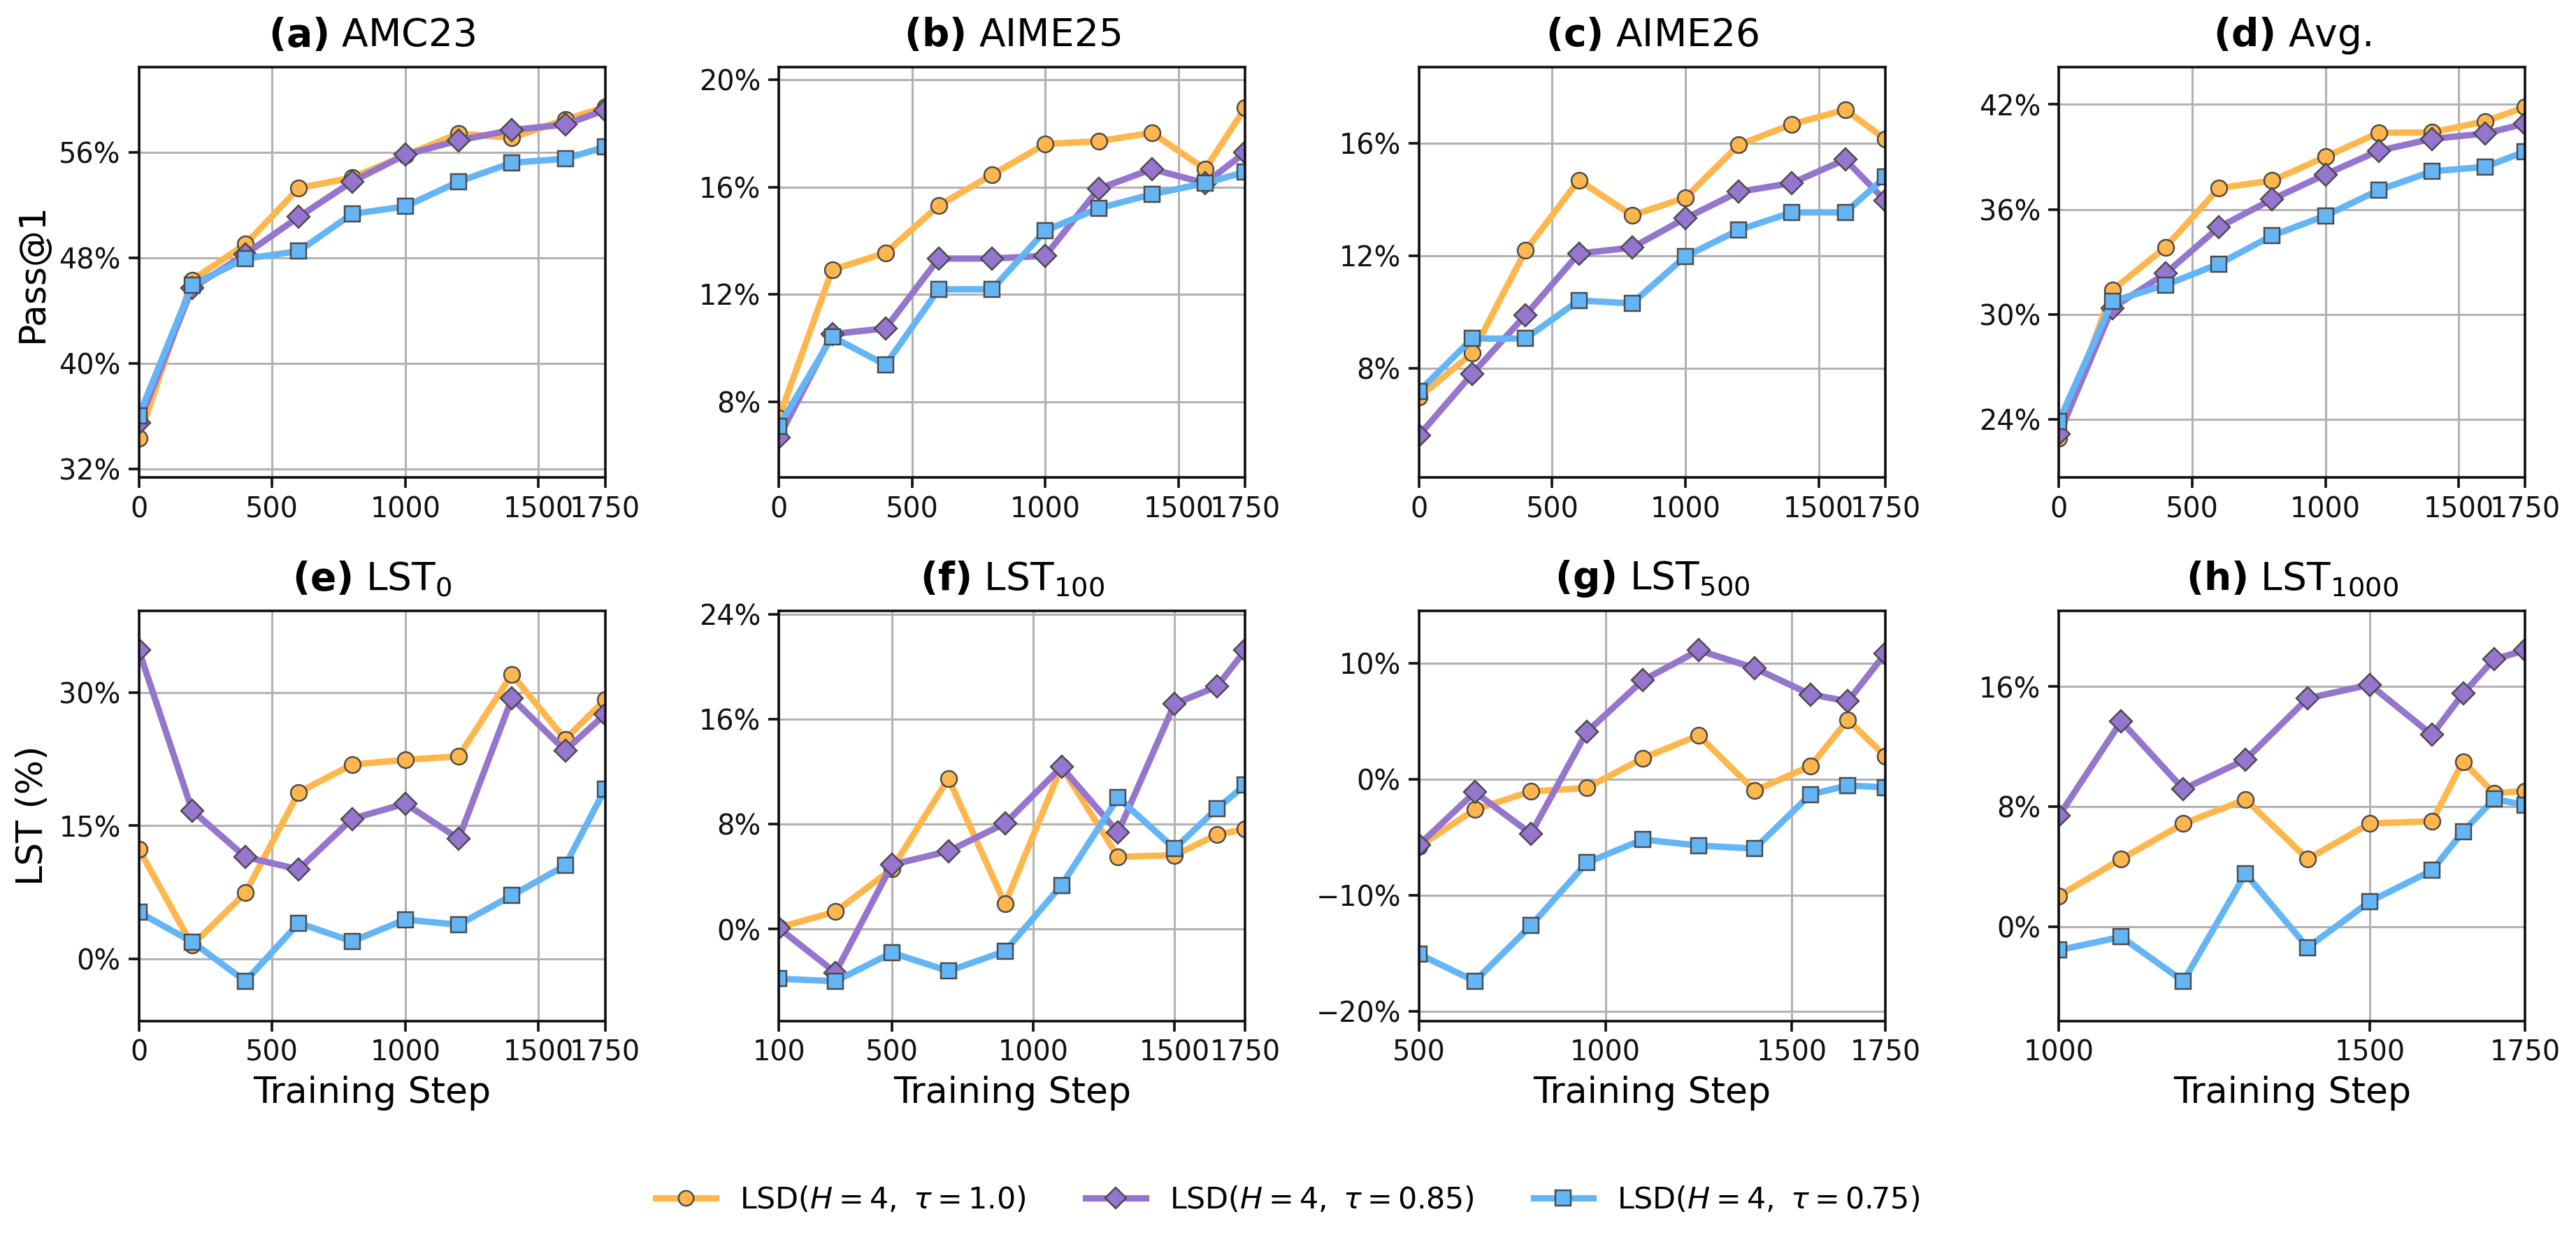
\includegraphics[width=0.80\linewidth]{figures/ablation_tau.png}
  \caption{\textbf{Routing-threshold ablation.} We compare $\tau=1.0,0.85,0.75$ at $H=4$ through step 1750. Panels follow Figure~\ref{fig:ablation-half-life}.}
  \label{fig:ablation-threshold}
\end{figure}

% The barrier after Conclusion allows these figures to share its page.
